\documentclass[12pt,a4paper,titlepage]{article}

\usepackage{preamble}

\title{Problème inverse en ElectroEncéphaloGraphie (EEG)}
\author{Saâd Aziz Alaoui, Yassine Jamoud, Samy Haffoudhi}
\date{\today}

\begin{document}

\maketitle

\section*{Introduction}

% sv pour accélèrer inversion (inverse des élements diagnoaux à la place du calcul entier)
% contrairement aux autres méthodes le filtre de tykinov n'a pas besoin de s

Lors de ce TP, nous allons nous intéresser à un exemple de problème
inverse dans le domaine biomédical : la localisation de sources en EEG.
Nous allons reconstruire l'activité à partir de mesures en surface par
les capteurs EEG.

On adopte la modélisation suivante :

$$ x(t) = G s(t) + n(t) $$

Avec,

\begin{itemize}
    \item{$ G \in \mathbb{R^{N \times D}} $}
    \item{N, le nombre de capteurs}
    \item{D, le nombre de dipôles de l'espace source}
    \item{$ x(t) \in \mathbb{R^N} $, le vecteur de mesures}
    \item{$ s(t) \in \mathbb{R^D} $, le vecteur de signal}
    \item{$ n(t) \in \mathbb{R^N} $, un vecteur de bruit}
\end{itemize}

Nous sommes face à un problème inverse linéaire et sous-déterminé
puisque $N \ll D$. Il convient alors de formuler des hypothèses
supplémentaires sur les sources pour obtenir une solution unique.
On utilisera dans ce TP la régularaisation de Tikhonov.

\section{Génération de données}

On travaille sur les données suivantes :

\begin{itemize}
    \item{$ D = 19626 $}
    \item{$ N = 91 $}
    \item{$ T = 200 $ échantillons}
    \item{Les signaux génèrrés proviennent de deux régions sources}
    \item{Le bruit est gaussien}
\end{itemize}

Affichons les signaux EEG pour 32 des 91 électrodes :

\begin{figure}[H]
    \caption{Signaux EEG bruités}
    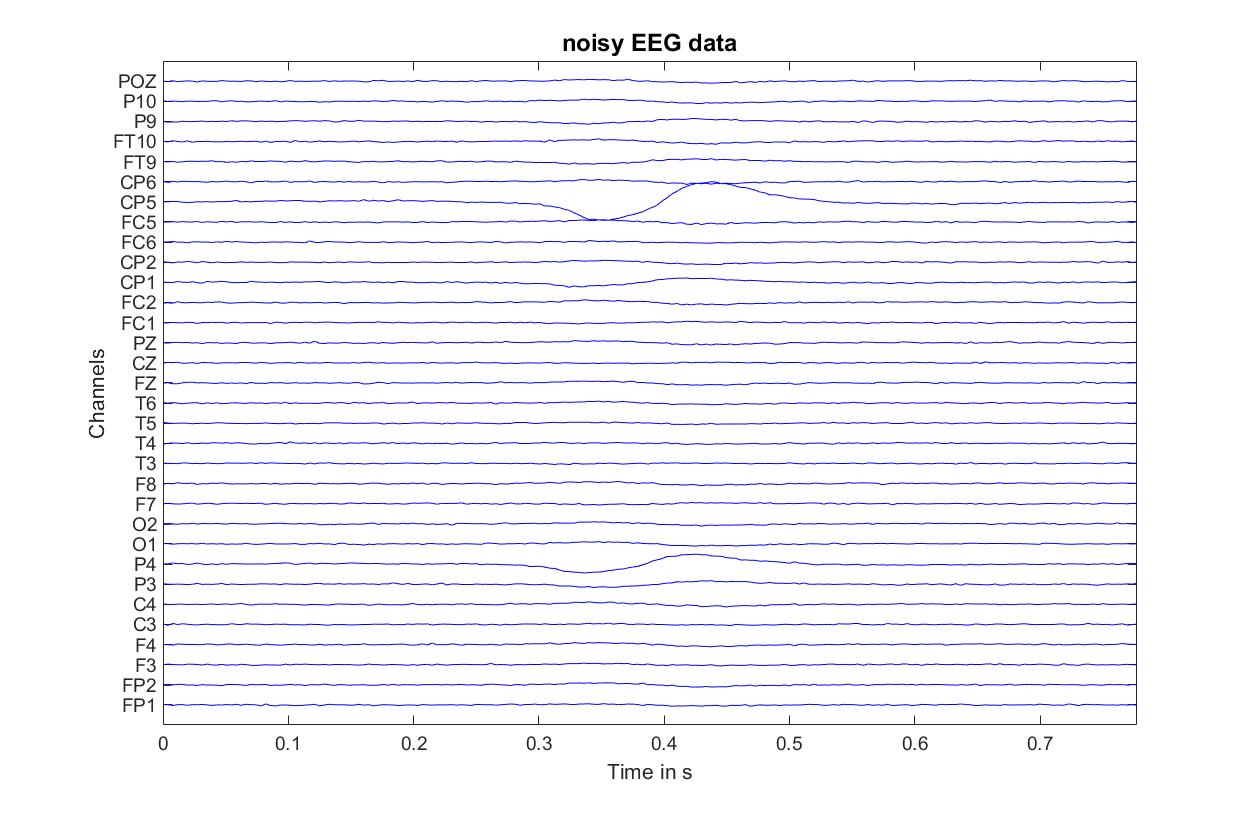
\includegraphics[width=.7\textwidth]{noisyEEG}
    \centering
\end{figure}

Et l'activité des dipoles de l'espace source :

\begin{figure}[H]
    \caption{Activité des dipôles}
    \label{brain}
    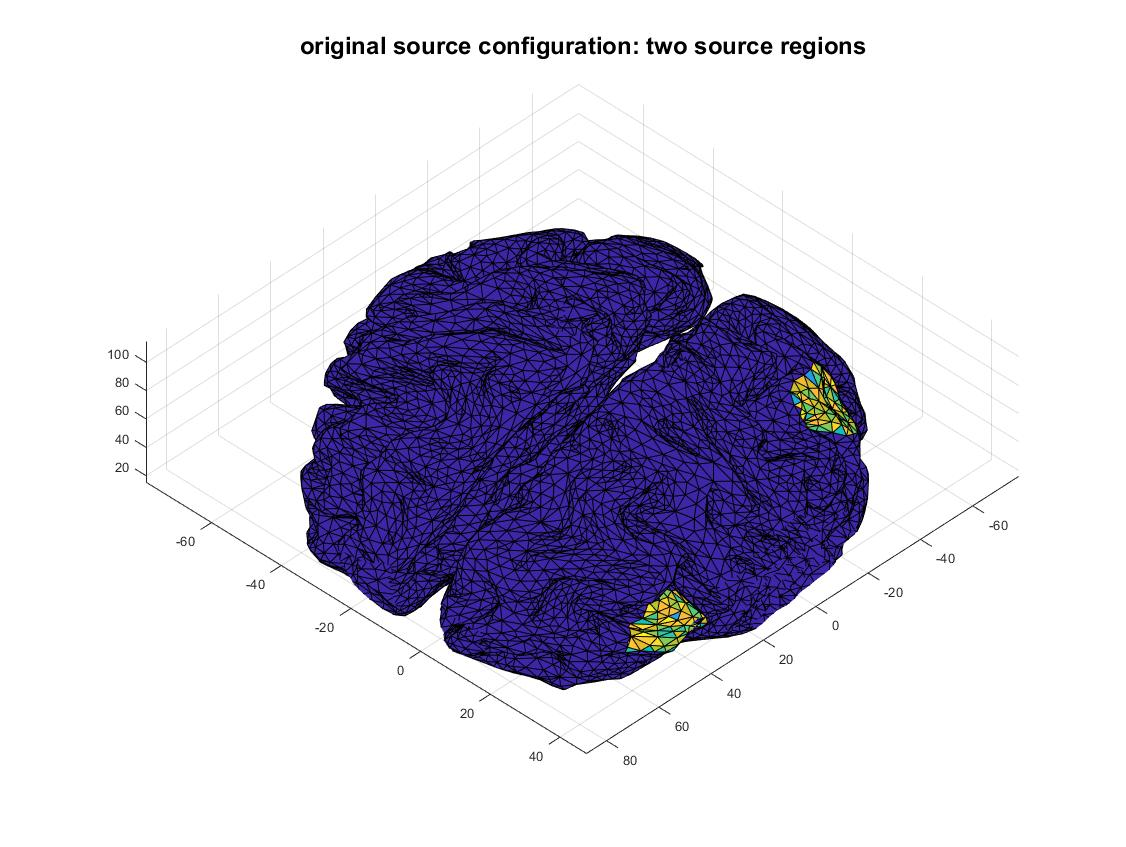
\includegraphics[width=.7\textwidth]{3dbrain}
    \centering
\end{figure}

On observe sur ces données des zones épileptiques quasiment similaires
au sein d'une me source distribuée ainsi qu'une activité de fond gaussienne.

Sur la figure \ref{brain}, on observe bien les deux régions sources
d'où proviennent les signaux générés. Nous allons comparer les résultats
obtenus plus tard à cette vérité terrain.

\section{Régularisation de Tikhonov}

La régularisation de Tikhonov consiste à ajouter un terme de régularisation
en norme 2 pour obtenir le problème d'optimisation suivant :

$$ \min \lVert x - Gs \rVert^2_2 + \lambda \lVert s \rVert^2_2 $$

Avec $\lambda$, un paramètre de régularisation et qui permet d'ajuster
le compromis entre l'adéquation au données et les hypothèses faites sur
la source.

On peut montrer par un calcul du gradient que la solution analytique vaut:

$$ s = G^t(GG^t + \lambda)^{-1}x $$

Par exemple, pour un rapport signal sur bruit égal à 10, affichons la
DLE (Distance Localisation Error)  en fonction de la valeur du
paramètre $\lambda$ :

\begin{figure}[H]
    \caption{RSB = 10}
    \label{lambdas}
    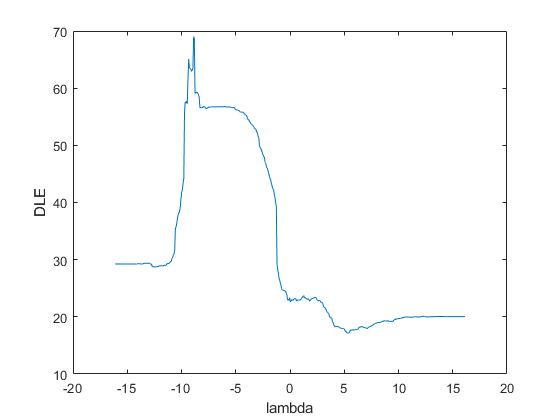
\includegraphics[width=.6\textwidth]{dle_lambda_03}
    \centering
\end{figure}

On balaye une large bande de valeurs du paramètre $\lambda$ et on
sélectionne celle qui permet de minimiser l'erreur DLE.

Affichons le résultat obtenu pour la valeur optimale de $\lambda$
pour trois valeurs différentes du RSB :

\begin{figure}[H]
    \caption{RSB = 0.1}
    \label{brain}
    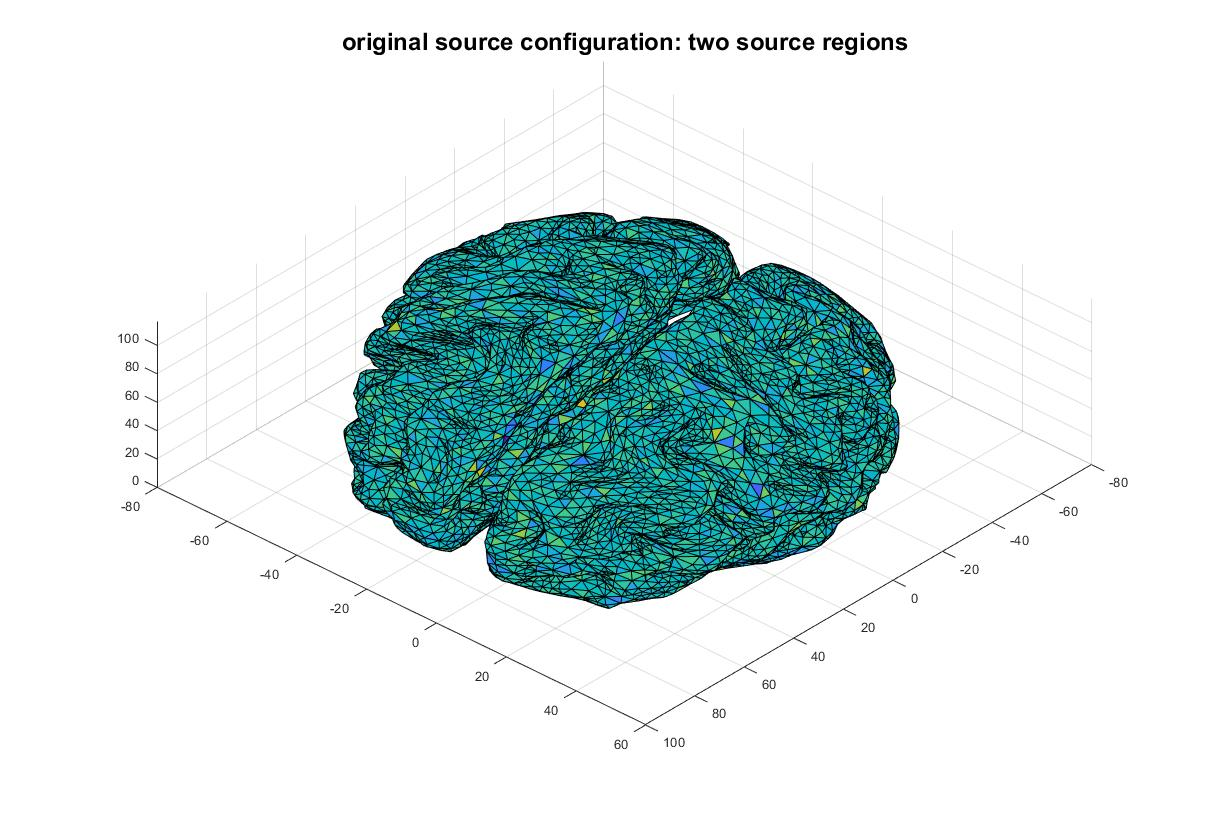
\includegraphics[width=.6\textwidth]{03_01_lambda_opti}
    \centering
\end{figure}

\begin{figure}[H]
    \caption{RSB = 10}
    \label{brain}
    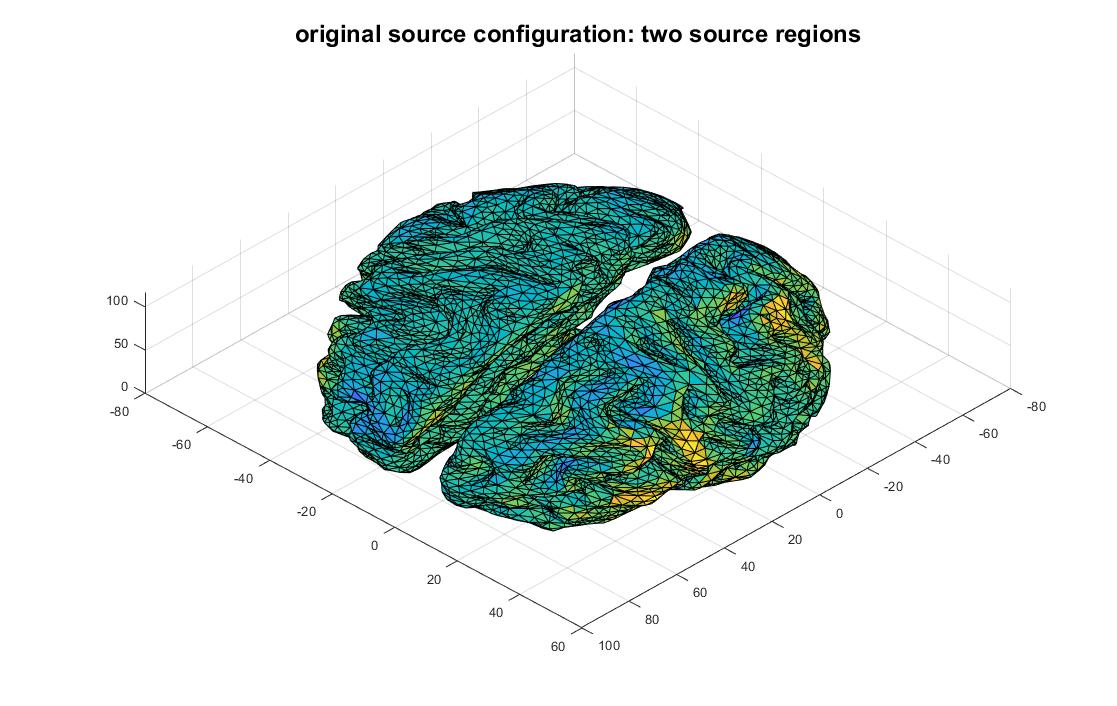
\includegraphics[width=.6\textwidth]{03_10_lambda_opti}
    \centering
\end{figure}

\begin{figure}[H]
    \caption{RSB = 100}
    \label{brain}
    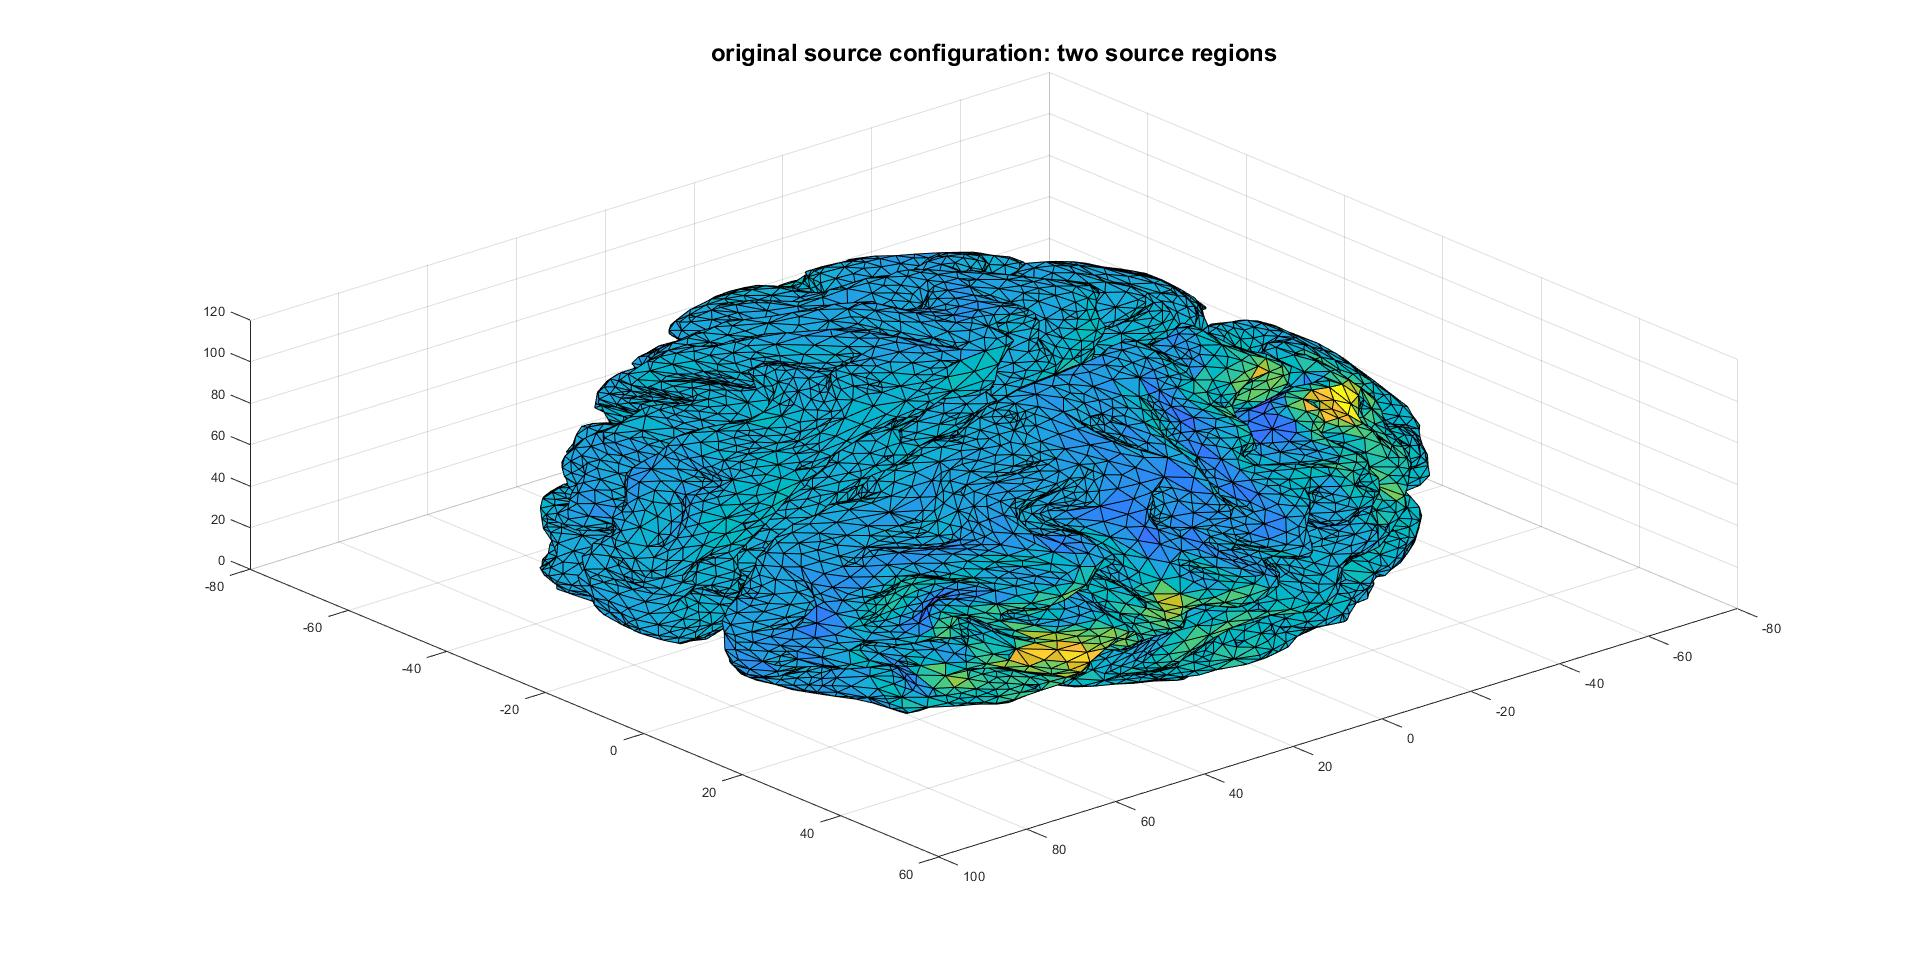
\includegraphics[width=.6\textwidth]{03_100_lambda_opti}
    \centering
\end{figure}

On obtient les valeurs suivantes :

\begin{itemize}
    \item{Pour un $RSB = 0.1$, $ \lambda_{opti} = 3.3 \times 10^{-5} $}
    \item{Pour un $RSB = 10$, $ \lambda_{opti} = 4298 $}
    \item{Pour un $RSB = 100$, $ \lambda_{opti} = 801 $}
\end{itemize}

On observe bien que :

\begin{itemize}
    \item{Plus on a de bruit, moins le résultat est proche de la vérité terrain.
        Pour RSB = 0.1, on ne distingue pas les sources, pour RSB = 10, on commence à distiguer
        les sources mais le résultat le plus proche est obtenu pour RSB = 100}
    \item{Les valeurs retournées pour $\lambda_{opti}$ différent entre les trois RSB et de manière non ordonnée,
        on ne peut donc pas exhiber un lien simple entre RSB et valeur de $\lambda_{opti}$.}
    \item{Comme on le voit par exemple sur la figure \ref{lambdas}, le choix de ce paramètre
        influe grandement sur la valeur DLE obtenue. Il faut donc faire attention à choisir une bonne valeur du paramètre
        si on veut obtenir des bons résultats.}
\end{itemize}

\section{L-curve}

Pour obtenir la meilleure valeur de $\lambda$,  on exploite alors
la L-Curve. Il s'agit du tracé de la norme de la solution en fonction
de la norme du résidu.

\end{document}
